\section{System Operation}
\label{sect:operation}
In order to construct a kit, the kitting system steps through each action in
the precomputed PDDL plan. Failures are searched for both before and after execution of 
each action. The overall process, known as {\sc BuildKit} is shown in Figure
\ref{fig:buildkit}. 

This process begins by retrieving a planning instance that has been 
precomputed to solve the construction of the requested kit (Line 1 of 
Figure \ref{fig:buildkit}). This is a high-level PDDL
plan that is not grounded to actual part instances or locations. It contains information
on the named storage location for classes of parts (individual SKU numbers), 
the quantity of each SKU that is required by the kit, and a build order (a sequence
of SKUs to be added to the kit). Additional information on the appropriate
end-of-arm tooling required to grip each part is also included.

This planning instance is decomposed into individual actions that must
be successfully carried out to complete the construction of the kit (the
{\it for} loop beginning at Line 2 of Figure \ref{fig:buildkit}). At this point,
preconditions of the action are examined to assure that the action to be attempted
is valid. If any of the action's preconditions are not able to be validated,
a failure is reported; otherwise, the action is approved for execution.
%
\begin{algorithm}[h!]
 \KwData{ $PredicateIn$ }
 \KwResult{true or false}
 	determine predicted pose $PoseR$ of $PredicateIn.ReferenceParameter$
 	and $PoseT$ of $PredicateIn.TargetParameter$ \;
 	send $PredicateIn$, pose $PoseR$, and $PoseT$ as focus of attention command to $SensorProcessing$\;
   	\uIf{$Eval(PredicateIn) == true$}{
 		return true\;
 	}
 	\Else{
 		return false \;
 	}
\caption{{\sc PredicateEvaluation} -- Returns the truth value of the predicate expression.}
\label{fig:predicateEval}
\end{algorithm}
%
\subsection{Precondition Validation}
\label{sect:preconditionValid}
Each precondition is a predicate expression that must be validated prior to
action execution.
The procedure for validating predicates is shown in Figure \ref{fig:predicateEval}. In Line 1 of this algorithm, the world
model is queried for the pose and class of each relevant 
parameter of the predicate. The information returned is the 
latest knowledge that has been recorded by the sensor processing
system and is not guaranteed to be up-to-date. This possibly out-of-date
information is used as a prediction of the object's current pose and the
knowledge is sent as a focus of attention indicator to the sensor
processing system. The sensor processing system is instructed to
update the world model with current observations
and to compute the supporting relationships necessary for predicate
evaluation.
%
\begin{algorithm}[h!]
 \KwData{ $PredicateIn, PoseR, PoseT$ }
 	determine actual pose $APoseR$ of $PredicateIn.ReferenceParameter$\;
 	determine actual pose $APoseT$ of $PredicateIn.TargetParameter$\;
 	determine RCC8 relations between $APoseR$ and $APoseT$\;
 	determine Intermediate State Relations based on RCC8 relations\;
 	determine truth value of $PredicateIn$ and write to MySQL database\;
\caption{{\sc SensorProcessing} -- Updates the MySQL database in the Execution world model
to contain the latest evaluation of predicates related to $PredicateIn$.}
\label{fig:sensorProcess}
\end{algorithm}
%
Figure \ref{fig:sensorProcess} depicts the algorithm that is followed by
sensor processing in the computation of predicate values. As may be seen from this
figure, the computation of predicates is a three step process that involves
the computation of increasingly complex forms of spatial relations. These
relationships; Region Connection Calculus (RCC8) relations, intermediate state relations, and predicate relations, are each represented as a separate class in
the ontology.
%
\subsubsection{RCC8 Relation --}
RCC8 \cite{Wolter2000} is an approach for representing the relationship between two regions in Euclidean or topological space. The class \class{RCC8\_Relation} 
is based on the definition of RCC8 and consists of eight possible relations that include Tangential Proper Part (TPP), Non-Tangential Proper Part(NTPP), Disconnected (DC), Tangential Proper Part Inverse (TPPi), Non-Tangential Proper Part Inverse (NTPPi), Externally Connected (EC), Equal (EQ), and Partially Overlapping (PO). In order to represent these relations in all three dimensions for the kitting domain, RCC8 has been extended to a three-dimensional space by applying it along all three planes (x-y, x-z, y-z) and by including cardinal direction relations ``+'' and ``-''. In the ontology, RCC8 relations and cardinal direction relations are represented as subclasses of the class \class{RCC8\_Relation}. 
%
\subsubsection{Intermediate State Relation --}
These relations can be inferred from the combination of RCC8 and cardinal direction relations. For  instance, the intermediate state relation \textbf{In-Contact-With} is used to describe that object \textit{obj1} is in contact with object \textit{obj2}. This is true if \textit{obj1} is externally connected to \textit{obj2} in the x-direction, the y-direction, or the z-direction,  and is represented with the following combination of RCC8 relations:
\begin{gather}
\textbf{In-Contact-With}(\textit{obj1}, \textit{obj2}) \rightarrow   \notag\\
\texttt{x-EC}(\textit{obj1}, \textit{obj2}) \vee \texttt{y-EC}(\textit{obj1}, \textit{obj2}) \vee \texttt{z-EC}(\textit{obj1},\textit{obj2}) \notag
\end{gather}
In the ontology, intermediate state relations are represented with the OWL built-in property \texttt{owl:equivalentClass} that links the description of the class \class{Intermediate\_State\_Relation} to a logical expression based on RCC8 relations from the class \class{RCC8\_Relation}.
\subsubsection{Predicate Relation --} The truth-value of predicates can be determined through the logical combination of intermediate state relations. The predicate \class{endeffector-location-endeffectorholder}(\textit{endeffector}, \textit{endeffectorholder}) is true if and only if the location of the end effector \textit{endeffector} is in the end effector holder \textit{endeffectorholder} and is not attached to a robot. This predicate can be described using the following combination of intermediate state relations:
\begin{gather}
\textsf{endeffector-location-endeffectorholder}(\textit{endeffector},\textit{endeffectorholder}) \rightarrow   \notag\\
\textbf{In-Contact-With}(\textit{endeffector}, \textit{enfectorholder}) \wedge \notag\\
\neg\textbf{In-Contact-With}(\textit{endeffector}, \textit{robot}) \notag
\end{gather}
As with state relations, the truth-value of predicates is captured in the ontology using the \texttt{owl:equivalentClass} property that links the description of the class \class{Predicate} to the logical combination of intermediate state relations from the class \class{Intermediate\_State\_Relation}.
\subsubsection{Truth Value Determination --}
As seen in Section \ref{sect:Ontology}, a predicate can have a maximum of two parameters. In the case where a predicate has two parameters, the parameters are passed to the intermediate state relations defined for the predicate, and are in turn passed to the RCC8 relations where the truth-value of these relations are computed. If the predicate has only one parameter, the truth-value of intermediate state relations, and by inference, the truth-value of RCC8 relations will be tested with this parameter and with every object in the environment in lieu of the second parameter. Our kitting domain consists of only one predicate that has no parameters. This predicate is used as a flag in order to force some actions to come before others during the formulation of the plan. Predicates of this nature are not treated in the concept of ``Spatial Relation''.

These truth values may be retrieved from the ontology for use in Line 3 of Figure
\ref{fig:predicateEval} which will then propagate back up to {\sc BuildKit}. If
the predicates are successfully evaluated, the action will be cleared for 
execution and a set of CRCL Commands will be 
generated.
%
\begin{figure}[htb!]
\begin{center}
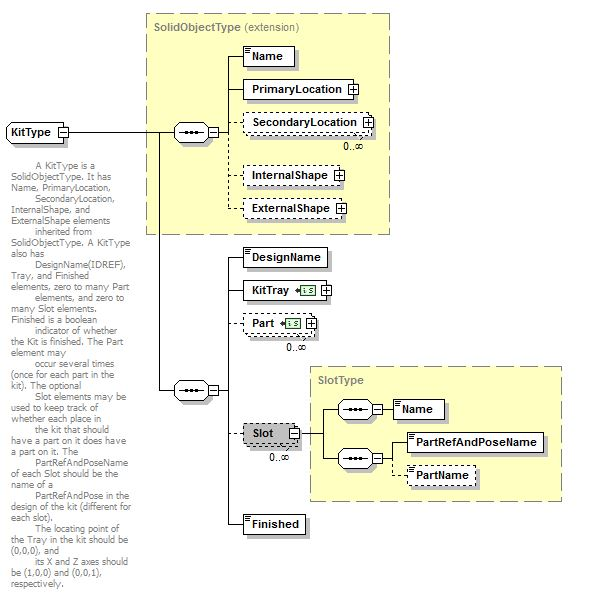
\includegraphics[width=12cm]{images/Kit.jpg}
\caption{Description of the KitType class that is designed to bring together
a container (the KitTray), a design for the kit creation, and specific parts
that populate the kit.}
\label{fig:kit}
\end{center}
\end{figure}
%
\subsection{Canonical Robot Command Language Generation}
Up to this point, the PDDL actions are not fully grounded to specific instances
that exist in the world. For example, the action \texttt{put-part} is designed
to place the part that is currently being held by the robot into a kit that
is specified as one of the action's input parameters. However, the precise
location for this part to be placed is not specified at the time of plan
creation. It is up to the Executor, working with the world model, to find
an empty slot in the kit that can receive the part. The structure of the
ontology is specifically designed to support this grounding, and this
structure is automatically replicated in the MySQL database that resides
in the Execution portion of the world model. 

Continuing with
the example of the \texttt{put-part} command, the Executor needs to find
an empty slot in the target kit to place the specific part that the robot is
holding. As shown in Figure \ref{fig:kit}, the {\sc KitType} class contains
zero to many {\sc Slot} classes that in turn contain specific location and 
part identification information. The Executor is able to read this information
from the world model and determine the precise global pose where the part
should be placed. The robot controller must now be commanded to complete this action.

While the action is an atomic element in PDDL, it will decompose into a series
of actions in CRCL. The robot will need to follow a safe trajectory to achieve
the slot in the kit, and the gripper will need to be controlled in order to release
the part. This one-to-many mapping is performed in the Executor and is currently
hand-coded for each of the PDDL commands that exists in the system. 
%
\subsection{Effect Validation}
The purpose of performing an action is to achieve results in the world. These results are represented in the PDDL effects. Each effect is a predicate expression that must be validated to assure proper
action execution. The technique for validating the effect predicates is identical
to the evaluation of the precondition predicates described in Section \ref{sect:preconditionValid}. If all of the effects are able to be validated, the
system will report the action's success and begin performing the next action in the plan.
%
\begin{figure}[htb!]
\begin{center}
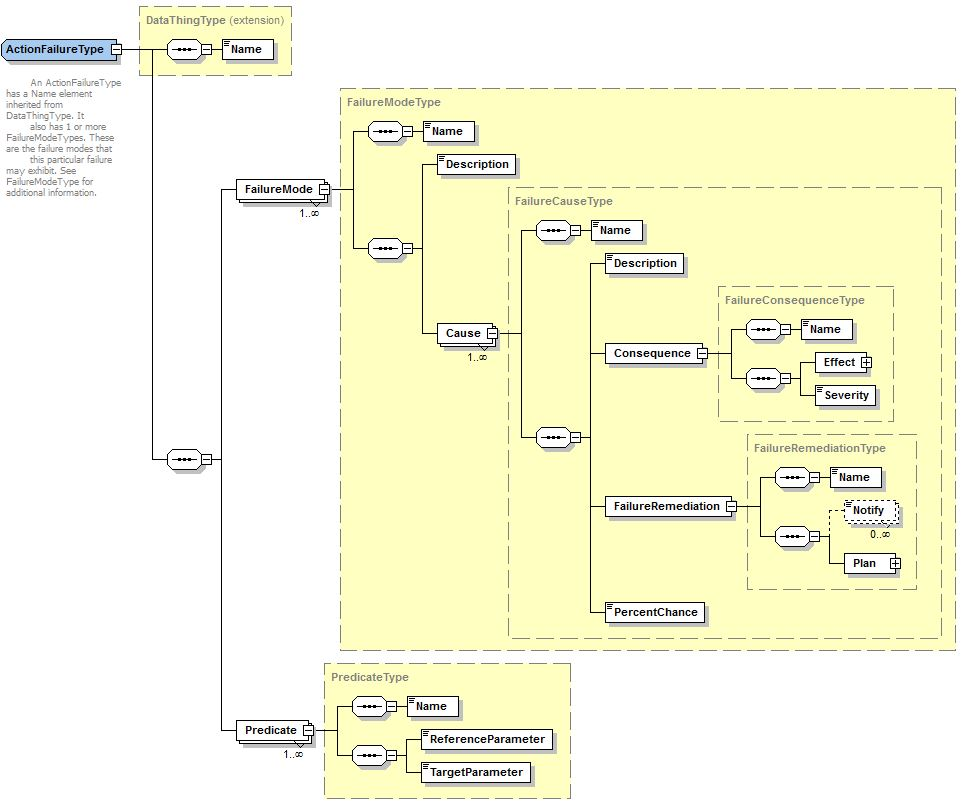
\includegraphics[width=12cm]{images/FailureType.jpg}
\caption{Description of the FailureType Class that is used to store information on action failures.}
\label{fig:failure}
\end{center}
\end{figure}
%